\section{Datenspeicherung im HDFS}

\subsection{Traditionelles Analysevorgehen}
In einem traditionellen Analysefall wäre als Beweismittel ein Datenträgerabbild des verdächtigen Computers erstellt worden. Mithilfe klassischer Opensource-Tools wie beispielsweise \textit{dd} kann damit zum Beispiel ein Image im RAW-Format erstellt werden. Andere Tools, wie beispielsweise \textit{FTK-Imager} können auch Datenträgerabbilder in speziellen Container-Formaten erstellen und lesen. Beispielsweise gibt es das \textit{EnCase Physical}-Format mit der Dateiendung \textit{e01}, oder das \textit{Advanced Forensic Format} mit der Endung \textit{.aff}.\footnote{Siehe \url{https://support.accessdata.com/hc/en-us/articles/222778608-What-Image-Formats-Do-AccessData-Products-Support-}, Stand: 4.4.2018.}.\\

\noindent
Einige Tools nutzen spezielle Container-Formate. Teilweise wird auch unterschieden, ob es sich um ein vollständiges Disk-Image handelt oder um ein logisches Dateiarchiv. Bei dem vollständigen Disk-Image werden auch nicht allokierte Speicherbereiche innerhalb des Dateisystems, der Partition oder des Datenträgers gesichert. Hier können sich potentiell versteckte und gelöschte Dateifragmente befinden. Mit diversen Tools kann ein sogenanntes File-Carving durchgeführt werden. Hierbei wird nur anhand der Rohdaten im Abbild versucht, Daten zu extrahieren. Die ist gerade auch dann sinnvoll, wenn nach gelöschten Dateien gesucht wird oder die Dateisystemmetadaten irreparabel beschädigt wurden.
\\ Ein logisches Dateiarchiv hingegen enthält wirklich nur die Dateien auf einer logischen Ebene und keine unallokierten Speicherbereiche. Von Vorteil hierbei ist eine geringere Speichergröße. Allerdings tritt durch die logische Sicherung ein potentieller Informationsverlust auf, da unallokierte Speicherbereiche nicht berücksichtigt werden, die aber dennoch potentiell auswertbare Informationen liefern könnten. Vertreter logischer Darteiarchive sind die allseits bekannten Archiv-Formate wie beispielsweise ZIP oder TAR.\\

\noindent
Letztlich werden die Beweismittel in unterschiedlichsten Formaten auf dem lokalen Analyse-Rechner gespeichert. Darauf aufbauend können die Daten in spezifische Formate konvertiert werden. Dies hängt aber meistens davon ab, wie sie weiter verarbeitet werden sollen und welche Werkzeuge zu dieser Verarbeitung genutzt werden.\\

\noindent
Im konkreten Testszenario ist das Datenträger-Abbild eines Linux-Rechners im RAW-Format auf dem lokalen Analyse-Rechner gespeichert. Das Abbild selbst kann ein oder mehrere Partitionen enthalten. Innerhalb der Partition werden Daten mithilfe unterschiedlicher Dateisysteme strukturiert gespeichert. Diese Dateisysteme können unter Windows mit dem Werkzeug \textit{X-Mount} oder unter Linux direkt mit dem Befehl \textit{mount} schreibgeschützt gemountet werden. Darauf wird das Dateisystem vom Betriebssystem interpretiert und als logisches Volume auf dem Analyse-Rechner bereitgestellt. Nun können die Dateien mit beliebigen Werkzeugen analysiert analysiert werden.\\

\noindent
In der Praxis hat das einfache schreibgeschützte Mounten den Vorteil, dass der Analyst relativ schnell im Dateisystem beliebige Dateien finden und dessen Inhalt mit diversen Tools anzeigen kann. Gerade für eine schnelle Vorprüfung ist dies sinnvoll. Im nachfolgenden Kapitel sollen nun Möglichkeiten zur Speicherung und Aufbereitung des Datenträgerabbildes mithilfe der forensischen Analyse-Plattform untersucht werden.


\subsection{Umsetzung in der Hadoop Analyse-Plattform}

Die Datenspeicherung im HDFS ist wohl der wichtigste Aspekt in dieser Thesis. Hierbei geht es nicht nur darum, wie das HDFS die Daten verwaltet sondern vielmehr um die Art und Weise, wie Daten forensisch korrekt gespeichert werden können.\\

\noindent
Der Standardfall wäre hierbei ein Rohdatenträgerabbild (RAW-Image), welches das Beweismittel darstellt. Hierbei liegen die Dateien als fragmentierte Blöcke in einer spezifischen Datenstruktur vor, welche das Dateisystem des Abbildes beschreiben. Je nachdem, ob ein Datenträgerabbild direkt von einer Partition eines Datenträgers oder vom ganzen Datenträger erstellt wurde, sind in dem Abbild unter Umständen auch mehrere Partitionen samt Partiationstabelle enthalten. Von diesen Partition kann wiederum jede einzelne Partition ein eigenes Dateisystem, wie beispiels FAT, ext4, oder NTFS enthalten. Dieses Dateisystem enthält dann die eigentlichen Dateien, welche logisch zusammengesetzt werden müssen.\\ Viele Linux-Distributionen bieten hier bereits eine weitreichende Unterstützung zum Lesen und Schreiben dieser Dateisysteme. Hierzu können die Dateisysteme einzelner Partitionen des Datenträgerabbildes \textit{gemountet} werden.\\

\noindent
Zur Speicherung der Daten im HDFS gibt es mehrere Möglichkeiten, deren Vor- und Nachteile nachfolgend dargestellt werden.

\subsubsection{Variante 1 - Datenträgerabbild im HDFS speichern}

Die naheliegende Variante zur Speicherung der Beweismittel, wäre die Datenträgerabbilder direkt im HDFS abzuspeichern. Allein die Größe der Abbilder wäre nicht problematisch. Um eine eine entsprechende Aufteilung kümmert sich das HDFS.\\ Allerdings hat die Lösung den entscheidenden Nachteil, bei der Weiterverarbeitung der Daten. Auf Betriebssystemebene lassen sich solche Datenträger einfach mounten. Zumal die meisten Betriebssysteme auch ein großen Teil der unterschiedlichen Dateisysteme auf einem Datenträger erkennen können. Aber innerhalb des Hadoop-Frameworks findet sich keine Unterstützung zum Lesen von beliebigen Dateisystemen. Denn normalerweise nutzen JAVA-Applikationen ein definierte Schnittstelle auf Basis logischer Dateien, die wiederum vom Betriebssystem bereitgestellt werden. Um die logischen Dateien aus dem Datenträgerabbild extrahieren zu können, müsste für jedes einzelnes Dateisystem eine eigene Implementierung geschrieben werden.\\ 
Darüber hinaus wäre das Extrahieren der Dateien aus einem Dateisystem auf einem Datenträgerabbild auch nicht wirklich performant. Angenommen das Auslesen würde mit Apache Spark durchgeführt werden. Aufgrund der eingangs beschriebenen Datenlokalität (siehe Kapitel \ref{ch:theory_hadoop}) wären auf jedem Knoten einzelne Blöcke von beispielsweise 128 MB Größe vorhanden. Um dann im ext4 Dateisystem eine Datei lesen zu können, sollten zumindest die Dateisystemmetadaten aus dem 1. Block in jedem Knoten verfügbar sein. Darüber hinaus können die Fragmente einer einzelnen Datei verstreut auf innerhalb des Dateisystems liegen. Je nach Fragmentierungsgrad des Dateisystem, müsste dann auf einem Data-Node in vielen Fällen weitere Blöcke anderer Knoten nachgeladen werden, da dort spezifische Fragmente der einzelnen Datei liegen könnten. Diese würde das Prinzip der Datenlokalität aushebeln. TODO: abbildung von ext4 dateisystem inklusive datei, welche überall verteilt ist. + letzter Absatz überarbeiten!


\subsubsection{Variante 2 - Logische Dateien im HDFS speichern}
Die zweite Variante wäre das Beweismittel auf dem lokalen Analyserechner zu mounten und alle Dateien auf logischer Ebene direkt in das HDFS zu importieren. 
Damit wäre die gesamte Dateisystemstruktur aus dem Datenträgerabbild im HDFS abgelegt. Allerdings wäre File Carving beziehungsweise das Auffinden von gelöschten Dateien nicht mehr im Hadoop-Framework möglich, sofern nicht auch der das Datenträgerabbild selbst nochmals in das HDFS importiert wird.\\ 

\noindent
Interessanter an dieser Variante ist aber das Verhalten des HDFS bezüglich der Metadaten und der unterschiedlichen Dateigröße. Bei dem Importierten müsste darauf geachtet werden, dass alle Metadaten des lokalen Dateisystem im Datenträgerabbild unverändert in das HDFS kopiert werden. 
Welche Metadaten bereits im HDFS mit angelegt werden, zeigt Abbildung \ref{fig:hdfs_file_properties} anhand eines Ausschnitts aus der Web-Repräsentation eines HDFS.\\
\begin{figure}[ht]
  \centering
  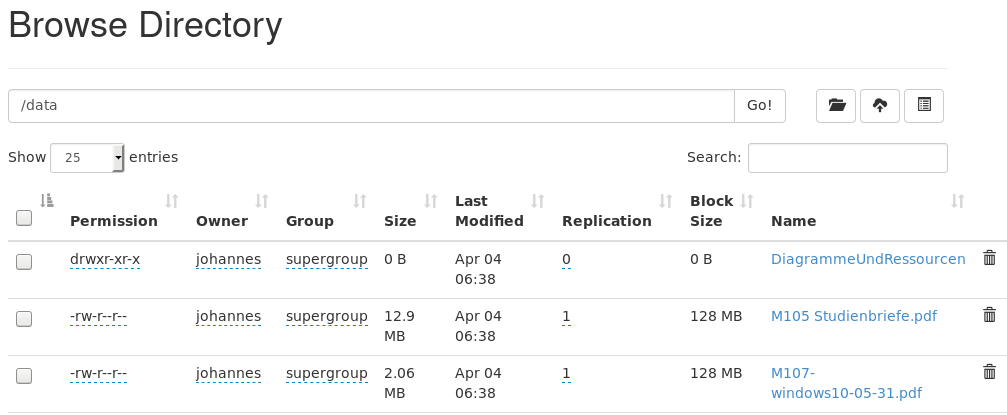
\includegraphics[width=\textwidth]{./resource/HDFS_FS_Example.png}
  \caption{HDFS - Dateieigenschaften}
  \label{fig:hdfs_file_properties}
\end{figure}

\noindent
Daraus ist ersichtlich, dass jede Datei entsprechende Dateirechte hat und einem Nutzer und einer Gruppe zugeordnet ist. Zusätzlich wird die Größe (nicht bei Verzeichnissen) und der Zeitstempel der letzten Änderung gespeichert. Die Anzahl der Replikationen und die Blockgröße sind spezifisch für das HDFS. Jede Datei kann auf einer unterschiedlichen Anzahl von Knoten repliziert sein. Die Standardkonfiguration definiert 3 Replikationen im realen Cluster, wobei Verzeichnisse nur logisch auf dem Name Node gehalten werden und damit auf keinem DataNode explizit repliziert werden. Auch die Blockgröße ist in der Standardkonfiguration auf 128 MB festgelegt. Wie im Grundlagenkapitel erwähnt, werden die Dateien in mehren Blöcken zu maximal 128 MB (konfigurationsabhängig) gespeichert und auch repliziert.\\ Bezogen auf klassische Dateisystem entspricht dies auch einem Block im ext4-Dateisystem oder einem Cluster im NTFS-Dateisystem (TODO: Quellenangabe!!! S.22 in M111). Es ist letztendlich die kleinste allozierbare Dateneinheit im Dateisystem. Dies bedeutet allerdings nicht, dass für jede Datei im HDFS auf den jeweiligen Date Nodes immer mindestens 128 MB Speicher belegt werden. Denn die reale Speicherbelegung auf dem Data Node beschränkt sich auch auf die reale Größe der Datei im lokalen Dateisystem des Data Nodes.\\

\noindent
Mit dem Befehl aus Listing \ref{lst:hdfs_put_command} können Dateien von einem lokalen Verzeichnis in das HDFS importiert werden. 
\begin{lstlisting}[label={lst:hdfs_put_command},caption= Befehl zum Speichern einer Datei im HDFS,captionpos=b,frame=single,style=customshell]
hdfs dfs -put test.pdf /test.pdf
\end{lstlisting}
Hierbei werden die ursprünglichen Metadaten der Datei nicht übernommen. So beschreibt der oben erwähnte Modifikationszeitstempel den Zeitpunkt, zu dem die Datei im HDFS das letzte Mal geändert wurde. Dies entspricht initial dem Import-Zeitpunkt. Auch werden Nutzer und Gruppenrechte nicht übernommen. Prinzipiell wäre es aber möglich die Metadaten aus dem lokalen Dateisystem mit in das HDFS zu übernehmen.\footnote{Hierzu kann dem \textit{put}-Befehl aus Listing \ref{lst:hdfs_put_command} der Parameter \textit{-p} mit übergeben werden.} Ratsam ist dies jedoch nicht, da gerade auch der Nutzer, die Gruppe und die dazugehörigen Zugriffsrechte in einem produktiven HDFS-Cluster verwendet werden, um Zugriffsbeschränkungen einzelner Nutzer und einzelner Programme umzusetzen.\\

\noindent
In der Theorie können noch weitere Metadaten gespeichert werden. Hierbei können erweiterte Dateiattribute beliebige Informationen über die Datei speichern. Mit nachfolgendenen Befehlen kann beispielsweise der originale Zeitstempel der Erstellung einer Datei hinzugefügt und ausgelesen werden. Hierbei kann der Name des Attributs und dessen Inhalt frei gewählt werden.
\begin{lstlisting}[label={lst:hdfs_fattr_command},caption= Befehl zum Hinzufügen und Auslesen von Metadaten,captionpos=b,frame=single,style=customshell]
# Create custom file attribute
hdfs dfs -setfattr -n user.ntfs.creationtime -v "2018-04-07T11:14:42,798583789+02:00" /test.pdf

# Read custom file attribute
hdfs dfs -getfattr -d -n user.ntfs.creationtime /test.pdf
\end{lstlisting}

\noindent
Mit dem obigen Befehl wäre es also prinzipiell möglich, Metadaten des ursprünglichen Dateisystems zu übernehmen. Allerdings müssen diese Metadaten zur Weiterverarbeitung zuerst für jede Datei im HDFS eingetragen werden.\\
Zusätzlich müssen beim Prozessieren der Daten mit Apache Spark die Metadaten auslesbar sein. Dieses Auslesen ist umständlich aber möglich.\footnote{Siehe Metadaten-Extraktion im Projekt \textit{foam-processing-spark} unter \url{https://github.com/jobusam/foam-processing-spark}.}\\ 
Letztlich ist es wohl aber auch ein Performance-Problem, denn diese Metadaten werden auf dem Namenode gespeichert.\footnote{Siehe \url{https://de.hortonworks.com/blog/hdfs-metadata-directories-explained/}, Stand 6.4.2018.} Somit müsste jeder Datanode diese Informationen wiederum explizit am Namenode anfragen.\\

\noindent
Das Fazit der Variante 2 lautet daher, dass die Dateimetadaten des originalen Datenträgerabbildes höchstens als erweiterte Attribute im HDFS abgelegt werden könnten. Beim Importieren müssten diese Metadaten bei jeder einzelnen Datei explizit nachgetragen werden. Pro Datei wäre dies nochmals ein eigener HDFS-Aufruf. Nicht zuletzt werden diese erweiterten Metadaten physikalisch im Namenode gespeichert. Dadurch benötigt der Namenode mehr Speicher. Viel schwerwiegender jedoch ist, dass die erweiterten Metadaten beim Prozessieren mit Spark angefordert werden müssten und somit der Namenode viel zu stark beansprucht werden würde.\\
Aus diesen Gründen ist die Variante 2 nicht akzeptabel. 

\noindent
TODO: weiterer Aspekt - performantes Prozessieren von vielen kleinen Dateien / bwz. Dateien unterschiedlicher Größe!!!\\

\subsubsection{Variante 3 - ZIP-File bzw. Hadoop Archive?}


\subsubsection{Variante 4 - Costum Forensic Format}
Metadaten,Blockaufteilung,logische Sicherung\\
nachteil, carving muss vorher passieren...

\subsubsection{Variante 5 - HBASE + HDFS}
Diese Variante beschreibt einen Ansatz, bei welchem die Metadaten und sehr kleine Dateien direkt in HBASE persistiert werden. Dateien größer XX MB werden direkt im HDFS abgelegt und im jeweiligen Dateieintrag in HBASE verlinkt. Auch hier müsste beim Import der Daten eine eigene Anwendung die Informationen aus dem Datenträgerabbild auslesen und entsprechend ihrer Struktur in HBASE und HDFS speichern.